\documentclass[xcolor=dvipsnames]{beamer}

\geometry{paperwidth=140mm,paperheight=105mm}

\usepackage[utf8x]{inputenc}
\usepackage{amsmath,amsfonts,amssymb}
\usecolortheme{default}
\usepackage{graphicx}
\usepackage{tikz}
\usepackage{caption}
\usepackage{nicefrac}
\usepackage{mathabx}
\usepackage{hyperref}
%\usepackage{wrapfig}
% %\usepackage{cutwin}

\definecolor{DarkBlue}{HTML}{002e77}

\newcommand{\averx}{\langle x \rangle}
\newcommand{\Raverx}{\averx_\mathrm{ren}}

\usetheme{Boadilla}
\usecolortheme[named=DarkBlue]{structure}
\useinnertheme{rounded}

\usefonttheme{professionalfonts}
\setbeamertemplate{navigation symbols}{}
\setbeamertemplate{enumerate items}[square]

\usepackage{algorithm}
\usepackage{algorithmicx}
\usepackage{algpseudocode}

\makeatletter
\renewcommand{\ALG@beginalgorithmic}{\small}
\makeatother

\usepackage{sourcecodepro}
\usepackage{listings}
\definecolor{mygreen}{rgb}{0,0.6,0}
\definecolor{mygray}{rgb}{0.5,0.5,0.5}
\definecolor{mymauve}{rgb}{0.58,0,0.82}
% \PassOptionsToPackage{svgnames}{xcolor}

\lstset{ %
  backgroundcolor=\color{white},   % choose the background color; you must add \usepackage{color} or \usepackage{xcolor}; should come as last argument
  basicstyle=\footnotesize\ttfamily, % the size of the fonts that are used for the code
  breakatwhitespace=false,         % sets if automatic breaks should only happen at whitespace
  breaklines=true,                 % sets automatic line breaking
  captionpos=b,                    % sets the caption-position to bottom
  commentstyle=\color{mygreen},    % comment style
  deletekeywords={...},            % if you want to delete keywords from the given language
  escapeinside={\%*}{*)},          % if you want to add LaTeX within your code
  extendedchars=false,              % lets you use non-ASCII characters; for 8-bits encodings only, does not work with UTF-8
  frame=single,	                   % adds a frame around the code
  keepspaces=true,                 % keeps spaces in text, useful for keeping indentation of code (possibly needs columns=flexible)
  keywordstyle=\color{blue},       % keyword style
  language=C,                      % the language of the code
  morekeywords={*,...},            % if you want to add more keywords to the set
  numbers=none,                    % where to put the line-numbers; possible values are (none, left, right)
  numbersep=5pt,                   % how far the line-numbers are from the code
  numberstyle=\tiny\color{mygray}, % the style that is used for the line-numbers
  rulecolor=\color{black},         % if not set, the frame-color may be changed on line-breaks within not-black text (e.g. comments (green here))
  showspaces=false,                % show spaces everywhere adding particular underscores; it overrides 'showstringspaces'
  showstringspaces=false,          % underline spaces within strings only
  showtabs=false,                  % show tabs within strings adding particular underscores
  stepnumber=1,                    % the step between two line-numbers. If it's 1, each line will be numbered
  stringstyle=\color{mymauve},     % string literal style
  tabsize=2,	                   % sets default tabsize to 2 spaces
  moredelim=**[is][\color{red}]{!@}{!@},
  %title=\lstname                   % show the filename of files included with \lstinputlisting; also try caption instead of title
}

\renewcommand{\UrlFont}{\small}

\newcounter{lecturecounter}
\setcounter{lecturecounter}{1}

\author[B. Kostrzewa]{Bartosz Kostrzewa, Ferenc Pittler, Martin Ueding, Carsten Urbach}
\title{C-Kurs Physik, 2017}
\institute[HISKP]{HISKP, Rheinische Friedrich-Wilhelms-Universität Bonn}
% \titlegraphic{\roundbox{\includegraphics[height=2cm]{UniBonn_CRC110_ETMC_INFN}}}
\date[April 2017]{April 2017}

\begin{document}

% \frame{}
\begin{frame}
 \titlepage
\end{frame}

\begin{frame}{Administrativa}
  \begin{itemize}
  \item{Vorlesung 03.04-13.04, 10-12 Uhr, \textbf{PI HS1}}
  \begin{itemize}
    \item{06.04: \textbf{HS HISKP} }
  \end{itemize}
  \vspace{0.2cm}
  \item{Bartosz Kostrzewa, bartosz\_kostrzewa@fastmail.com, Raum 3.009 HISKP}
  \begin{itemize}
    \item{Sprechzeiten: Täglich 17:00-17:45 Uhr}
  \end{itemize}
  \vspace{0.2cm}
  \item{Tutoren}
  \begin{itemize}
    \item{Martin~Ueding, Simon~Schlepphorst, 
         \\Ferenc~Pittler, Marcel~Nitsch, Florian~Tauber} 
  \end{itemize}
  \vspace{0.2cm}
  \item{Tutorien finden statt: täglich 13:00-17:00}
  \begin{itemize}
    \item{Astro CIP Pool (Raum 0.007) [AifA, Auf dem Hügel 71]}
    \item{HISKP SR1 [HISKP, Nußallee 14-16]}
    \begin{itemize}
      \item{\textbf{ $\mathbf{18}$ Personen $\rightarrow$ Astro, $\quad\mathbf{N-18}$ $\rightarrow$ SR1} }
    \end{itemize}
  \end{itemize}
  \vspace{0.2cm}
  \item{Das Skript dient als Referenz und sollte zumindest während der Tutorien befragt werden!}
  \vspace{0.2cm}
  \item{Fundamentale Ungleichung der Programmierung (FUP!): \\ \textbf{Praxis $\mathbf{\gg}$ Vorlesungen} $\rightarrow$ besuchen Sie die Übungen, sonst bringt die Vorlesung nichts!}
  \item{Folien, Übungszettel, Beispielprogramme: \textcolor{blue}{\url{http://goo.gl/xhJN08}}}
  \end{itemize}
\end{frame}

\begin{frame}{Lernziele}
\begin{itemize}
  \item{Algorithmen verstehen und entwickeln}
  \item{Algorithmen in Quelltext übertragen}
  \vspace{0.3cm}
  \item{Erstes Kennenlernen der sogennanten \emph{imperativen} Programmierung}
  \item{Kennenlernen der Daten- und Kontrollstrukturen von C99}
  \vspace{0.3cm}
  \item{Praktischer Einsatz des C-Compilers zur Übersetzung des Quelltextes in ausführbaren Maschinencode}
  \item{Erstellen eigener C-Programme in den Tutorien}
  \begin{itemize}
    \item{einfache Beispielprogramme $\rightarrow$ kompliziertere Programme aus merheren Quelltextdateien}
    \item{Verwendung externer Bilbiotheken}
  \end{itemize}
  \vspace{0.3cm}
  \item{Vorbereitung auf \emph{physik441: Computerphysik} (SoSe 2017), \emph{physics760: Computational Physics} (WiSe 2017/2018), etwaige Bachelor- und Masterarbeiten}
\end{itemize} 
\end{frame}

\begin{frame}{Anwendung: Plasmaphysik / Fusion}
  \centering
  Wellenstein 7-x Stellerator\\ \vspace{0.2cm}
  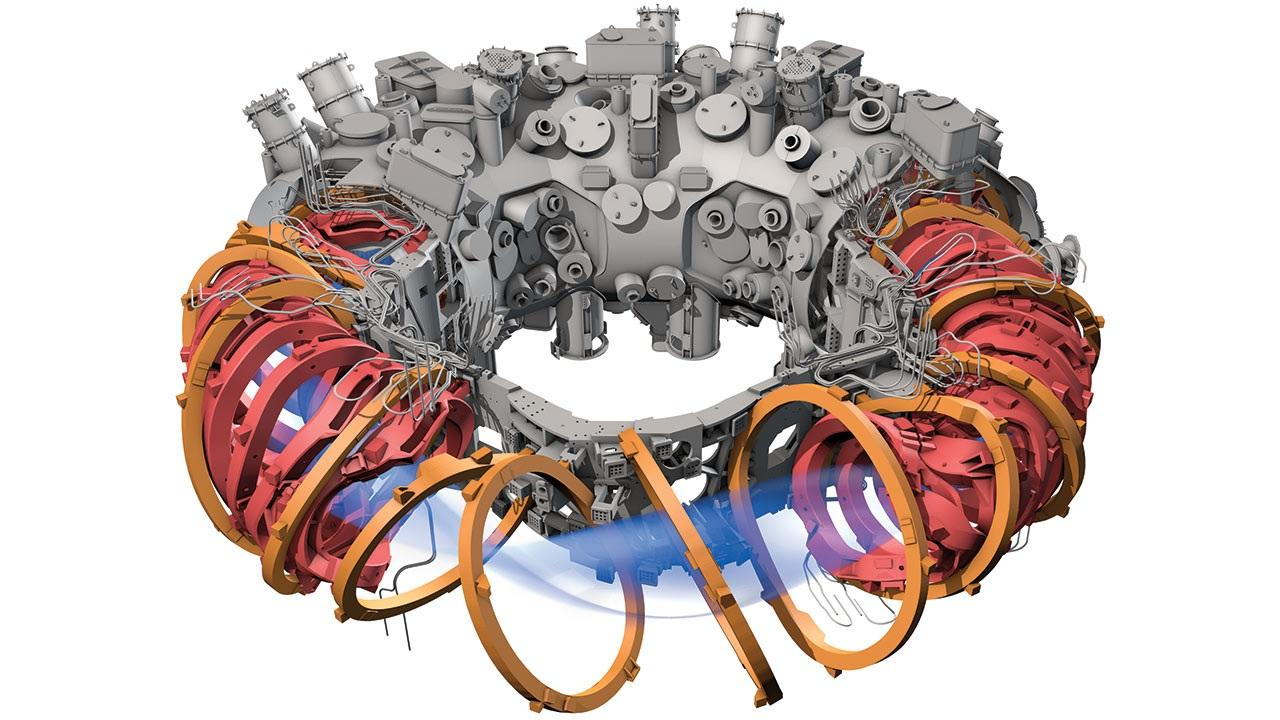
\includegraphics[width=0.9\textwidth]{graphics/stellerator.jpg}\\
  {\small Quelle: \url{http://www.sciencemag.org/news/2015/10/bizarre-reactor-might-save-nuclear-fusion} }
\end{frame}

\begin{frame}{Anwendung: Kosmologie / Astrophysik}
  \centering
  Simulation der Galaxie M74 über 13 Milliarden Jahre\\ \vspace{0.2cm}
  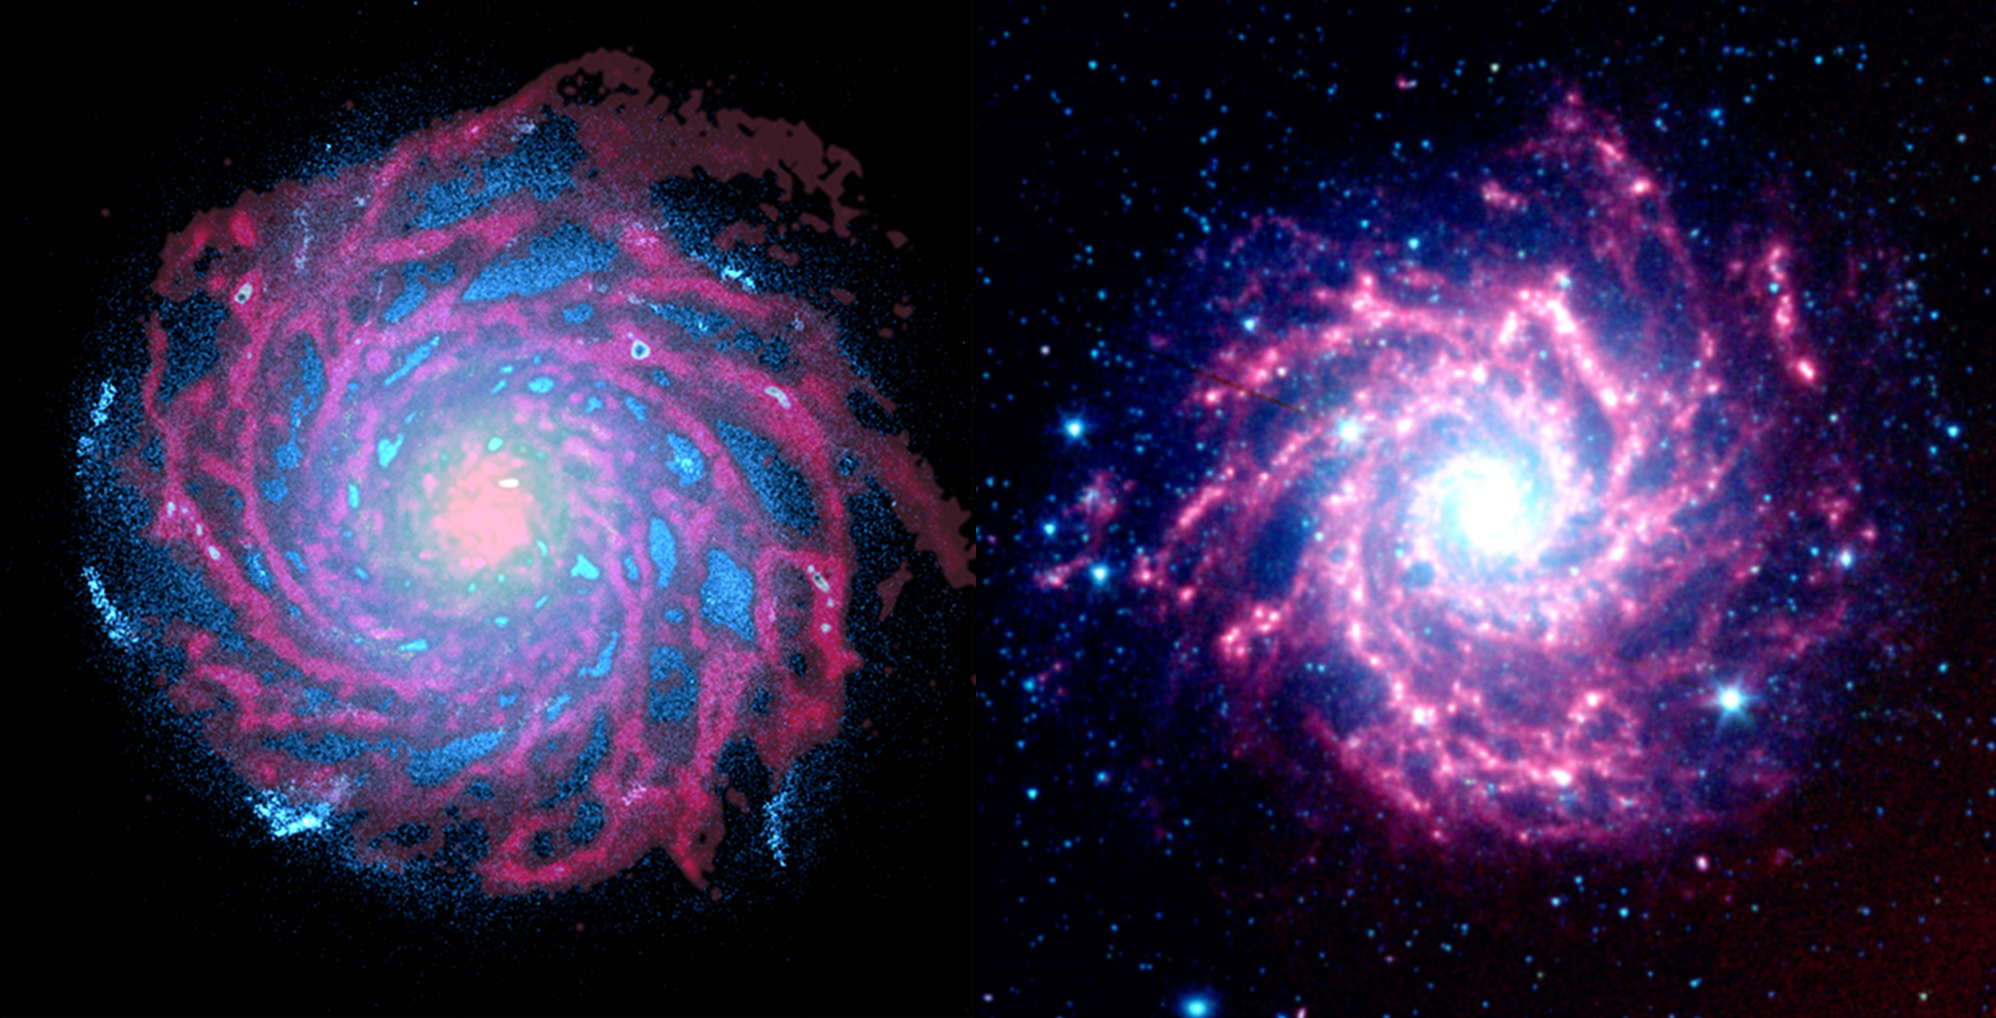
\includegraphics[width=0.9\textwidth]{graphics/m74_simulation.png}\\
  {\small Quelle: \url{http://www.hpc-ch.org/first-realistic-simulation-of-the-formation-of-the-milky-way-computed-at-cscs/} }  
\end{frame}

\begin{frame}{Anwendung: Hochenergiephysik - LHC}
  \centering
  Kollision im ATLAS-Experiment\\ \vspace{0.2cm}
  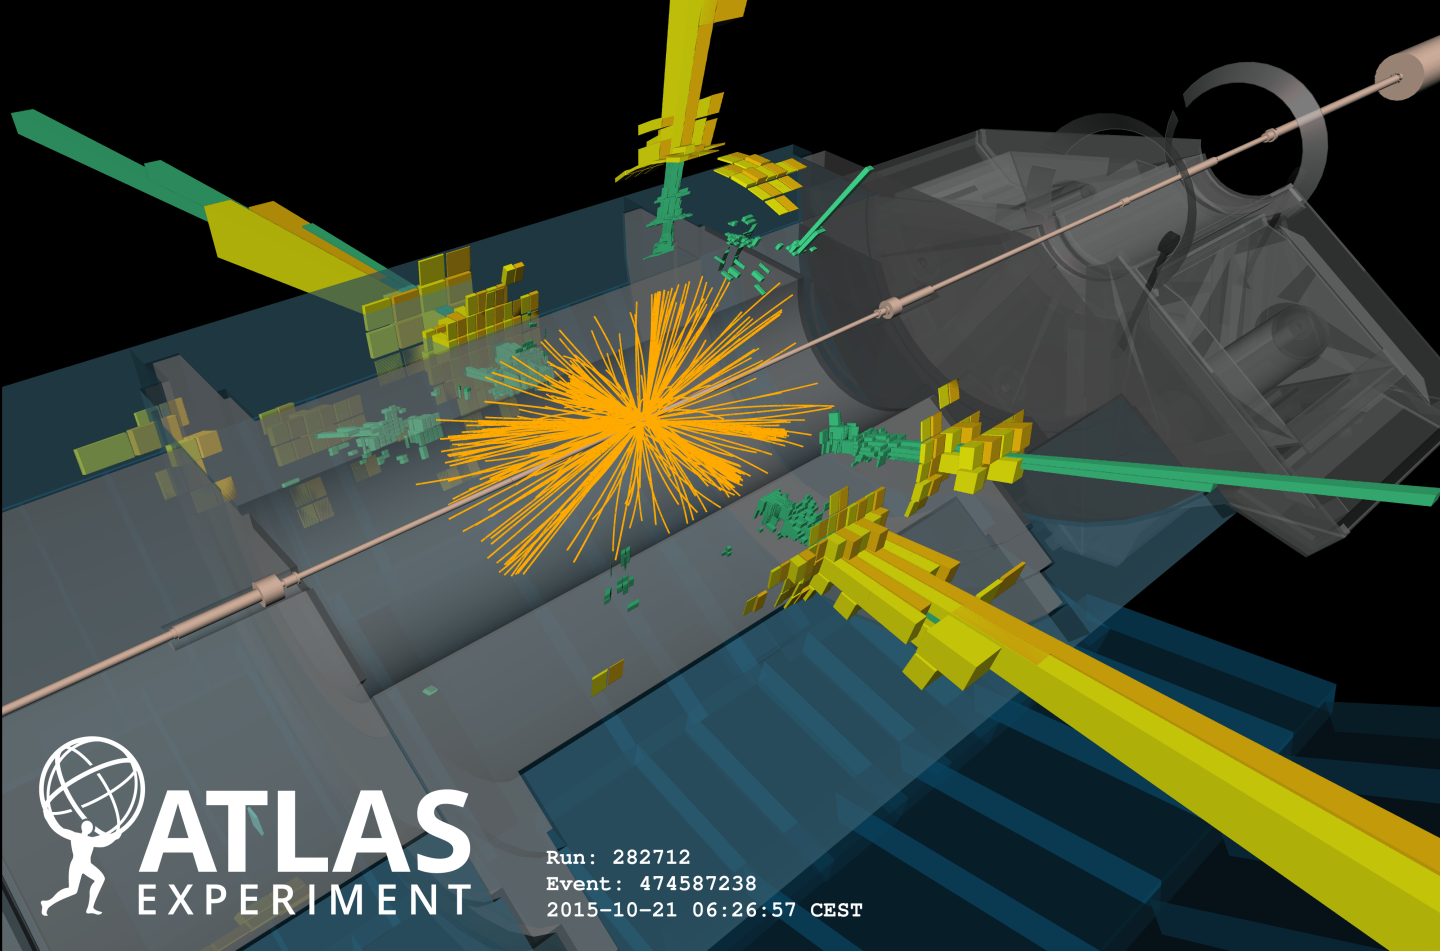
\includegraphics[width=0.9\textwidth]{graphics/atlas_event.png}\\
  {\small Quelle: \url{ https://cds.cern.ch/record/2113241 } }
\end{frame}

\begin{frame}{Anwendung: Hochenergiephysik / Gitter-QCD}
  \centering
  Simulation der Quantenchromodynamik auf Hochgeschwindigkeitsrechnern\\ \vspace{0.2cm}
  \begin{columns}
  \column{0.49\textwidth}
    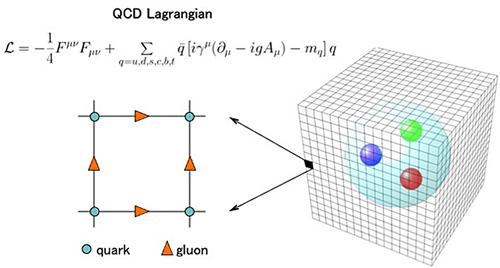
\includegraphics[width=0.8\textwidth]{graphics/LQCD2.jpg} \\
  \column{0.49\textwidth}
    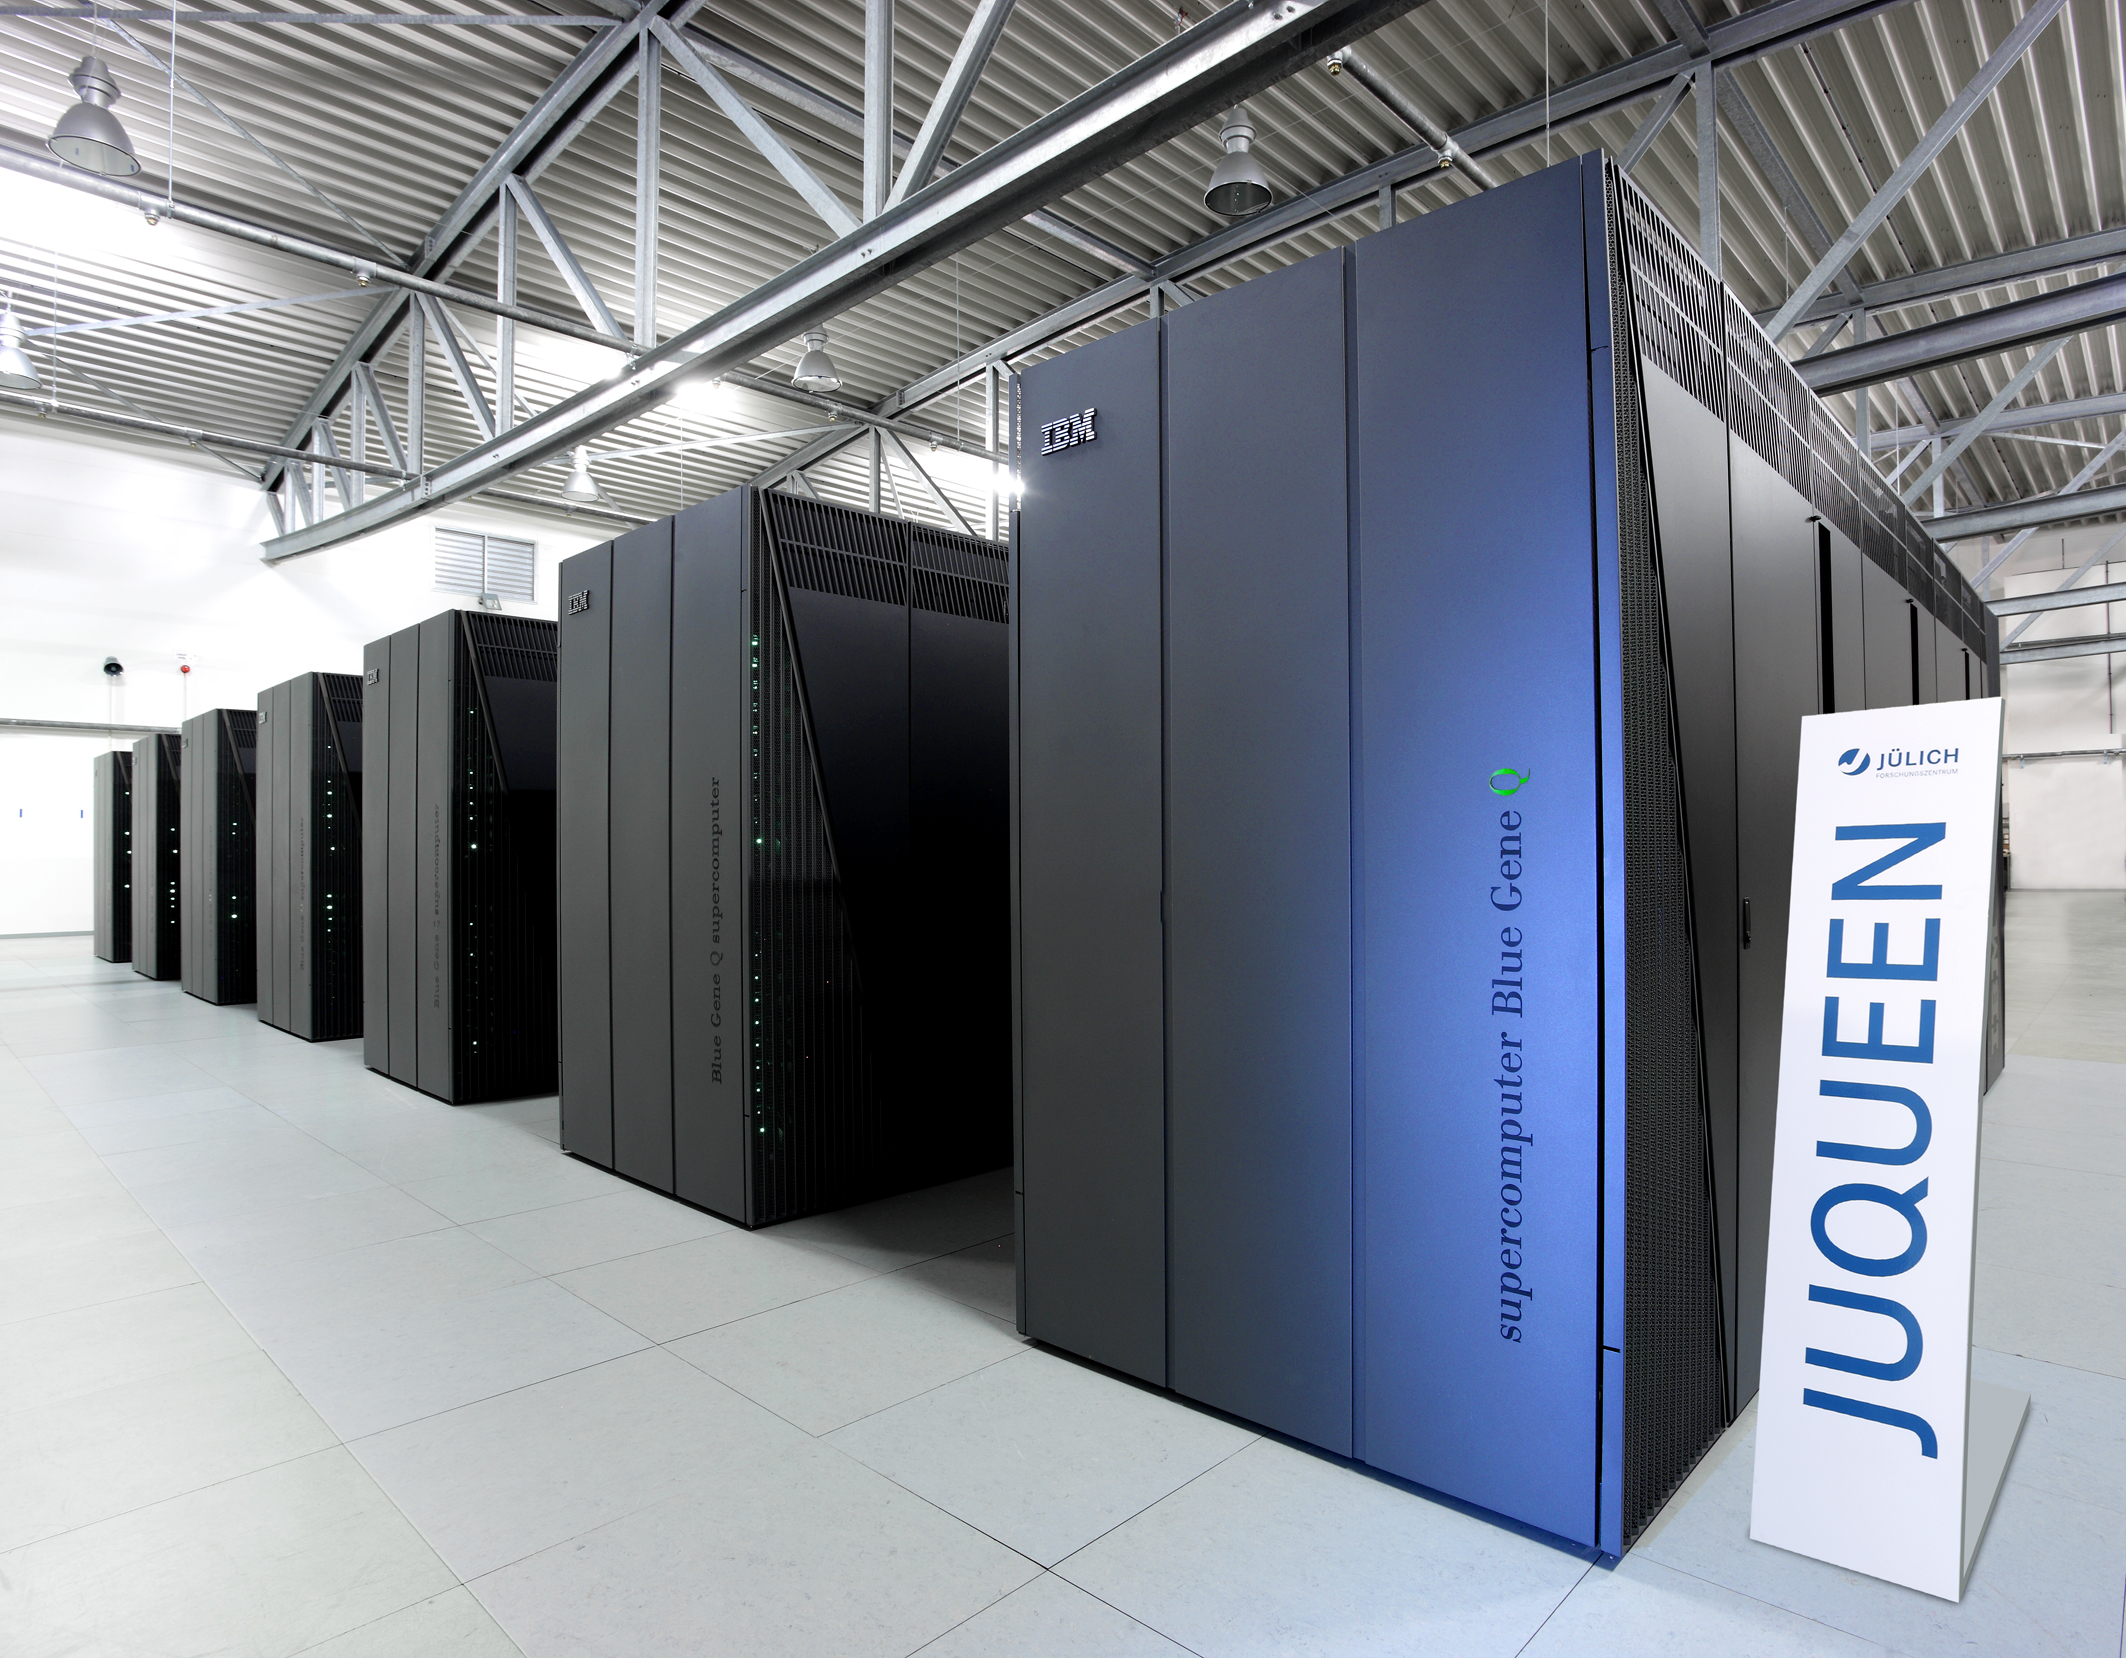
\includegraphics[width=0.8\textwidth]{graphics/juqueen.jpg} \\
  \end{columns}
  \vspace{0.3cm}
  {\small Quellen: \url{http://lpc-clermont.in2p3.fr/IMG/theorie/LQCD2.jpg} \\
                   \url{http://www.fz-juelich.de/ias/jsc/EN/Expertise/Supercomputers/JUQUEEN/JUQUEEN_node.html} }
\end{frame}

\begin{frame}{Anwendung: Biophysik / Biochemie - Molekulardynamik}
  \centering
  Simulation des NMDA Proteins und Rezeptors im menschlichen Gehirn\\ \vspace{0.2cm}
  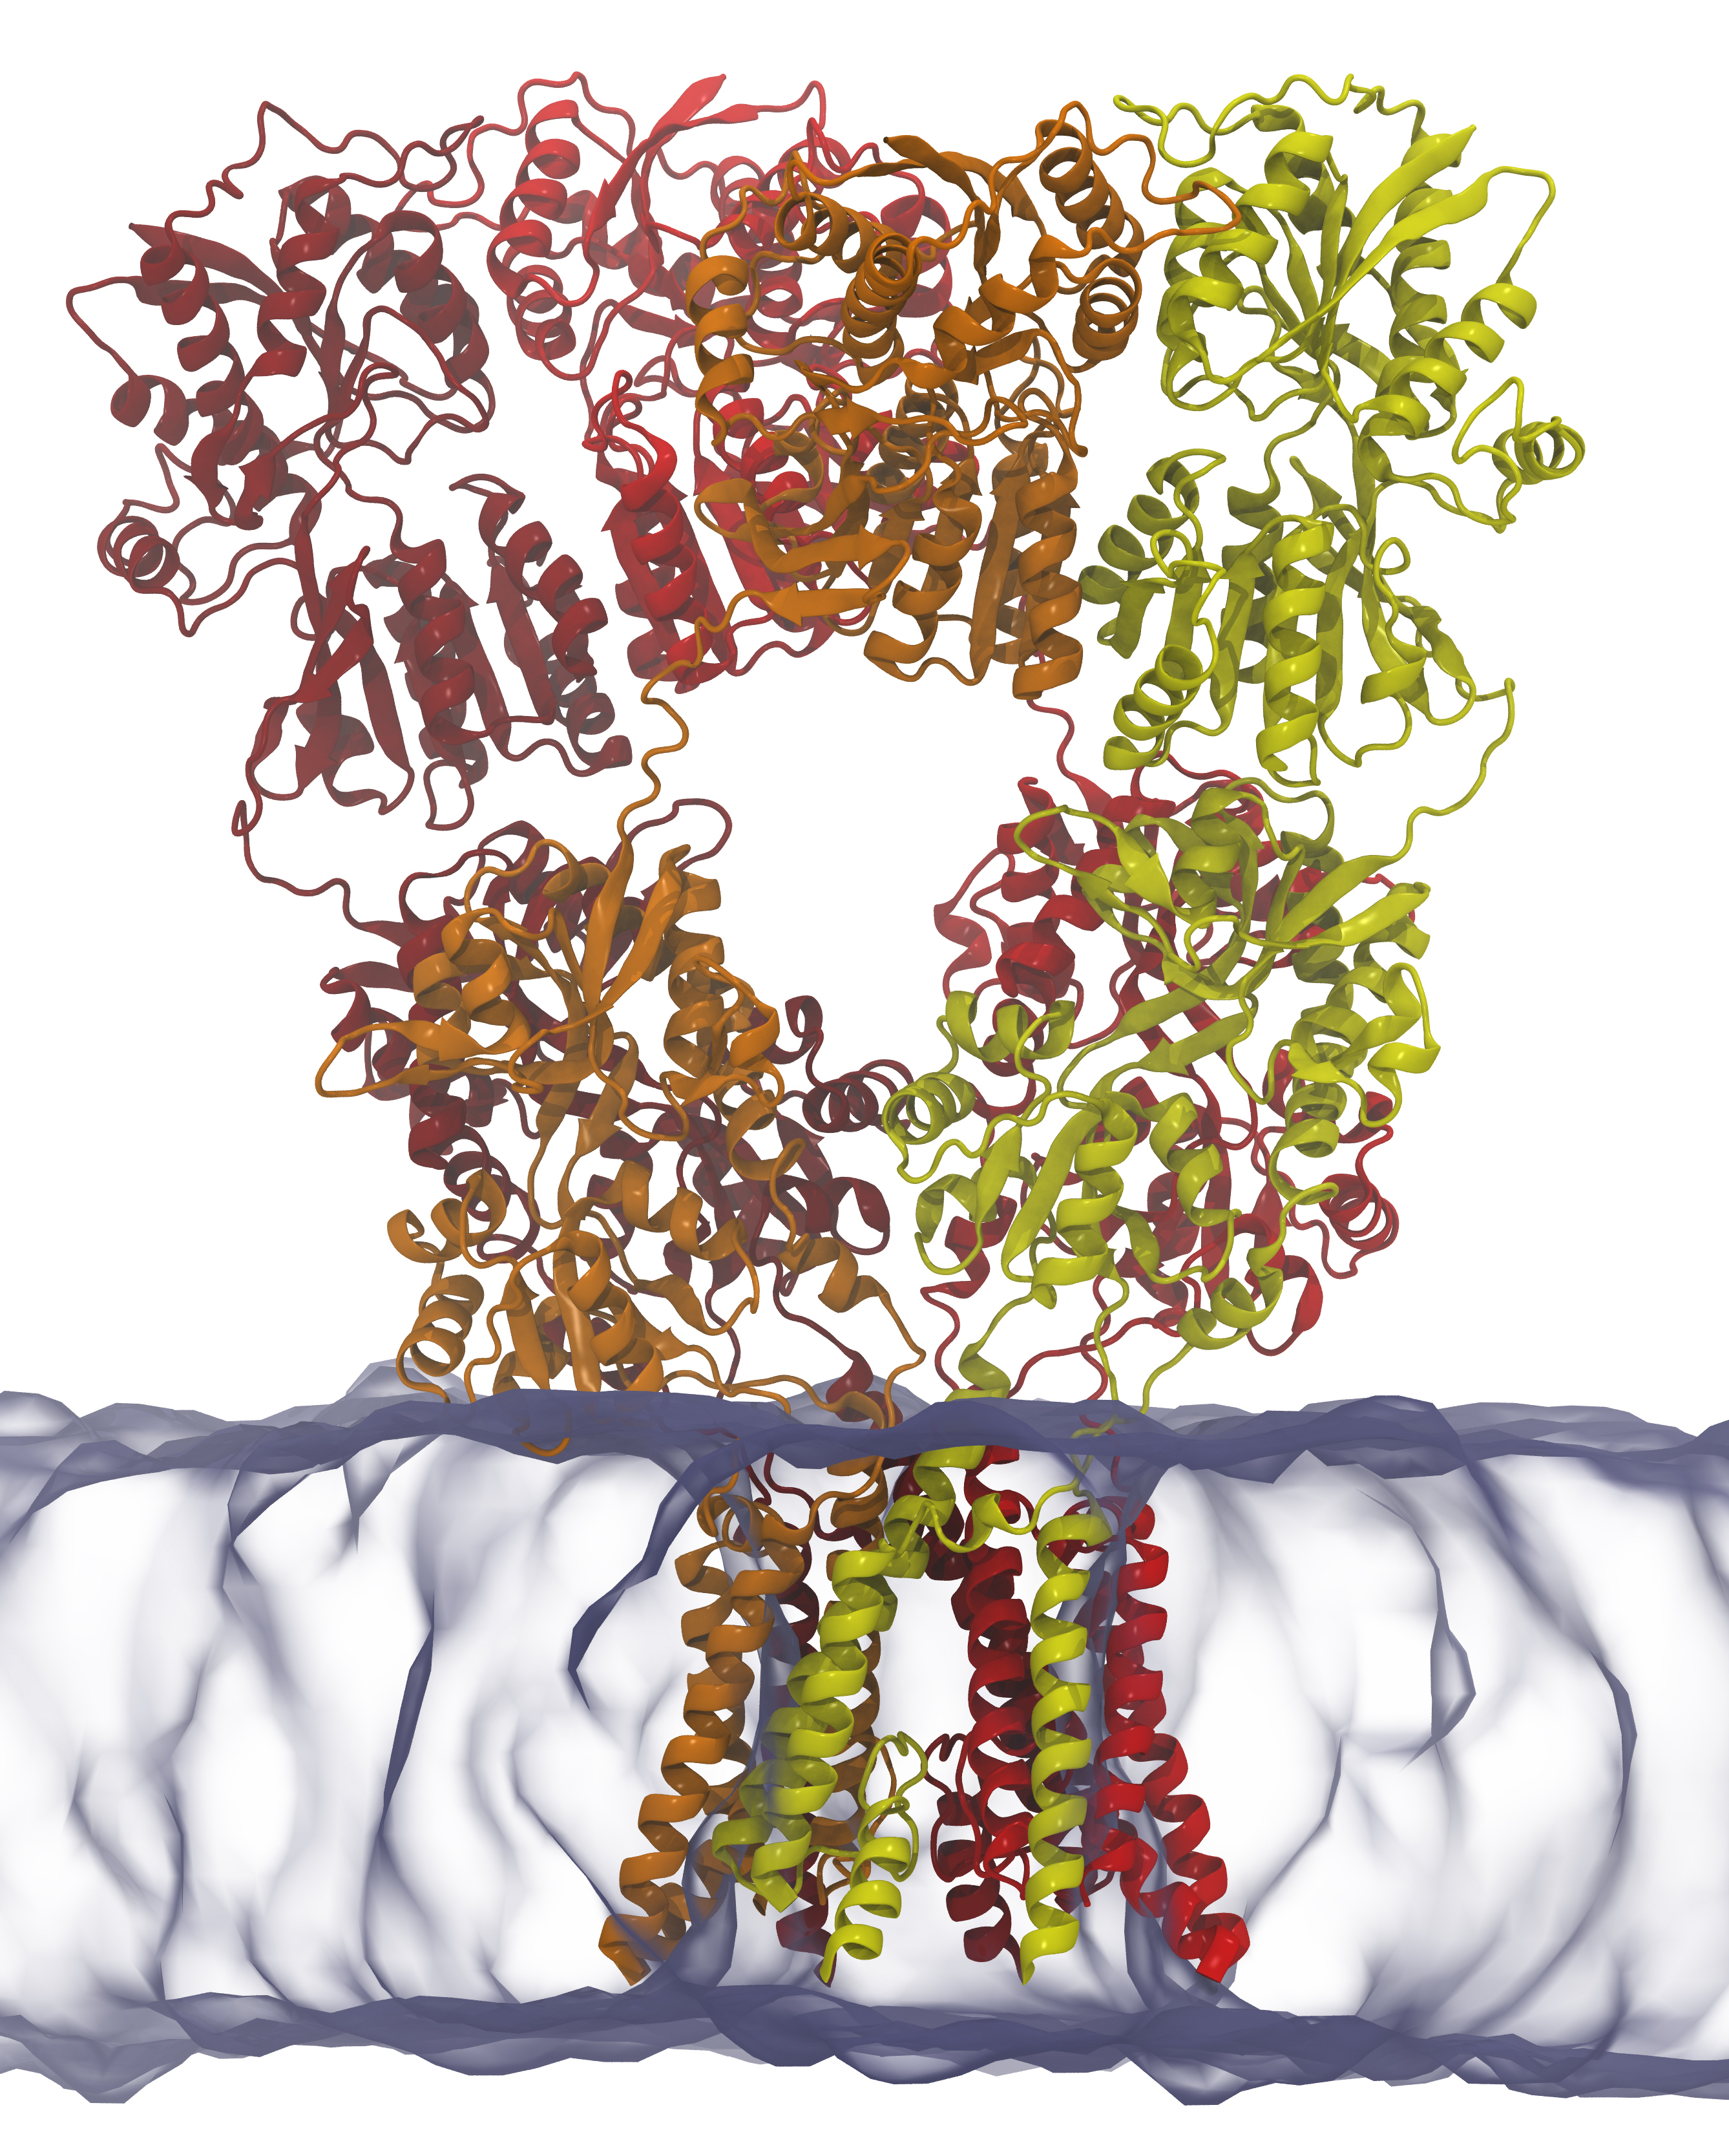
\includegraphics[width=0.4\textwidth]{graphics/glutamate.jpg}\\
  {\small Quelle: \url{http://computation.llnl.gov/glutamate-receptor-molecular-dynamics-simulation} }
\end{frame}

\begin{frame}{Die Programmiersprache C}{Vorlesung \arabic{lecturecounter}}
  \centering
  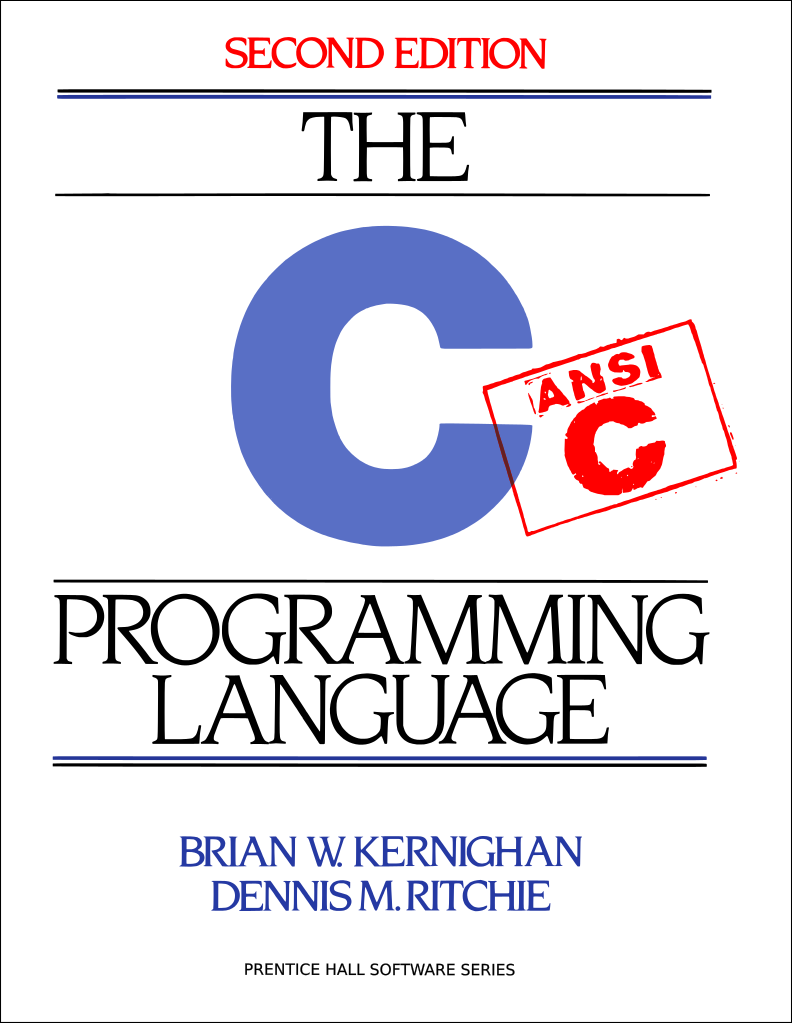
\includegraphics[height=7cm]{graphics/The_C_Programming_Language_cover}
\end{frame}

\begin{frame}{Algorithmus: Einfügensortieren Pseudocode}{Vorlesung \arabic{lecturecounter}}
  \begin{algorithmic}
  \Procedure{insertionsort}{$U,S$}
    \State \textbf{Input:} Lists $U,S$
    \State \textbf{Output:} List $S$
    \For {$i=0$ \textbf{to} \textbf{length}(U)-$1$}
      \State $S_i \gets U_i$
      \State $j \gets i$
      \While {$j > 0$}
        \If{ $S_j < S_{j-1}$}
          \State $t \gets S_j$
          \State $S_j \gets S_{j-1}$
          \State $S_{j-1} \gets t$
          \State $j \gets j-1$
        \Else
          \State \textbf{break}
        \EndIf
      \EndWhile
    \EndFor
  \EndProcedure
\end{algorithmic}

\end{frame}

\begin{frame}[fragile]{Die Struktur eines C-Programms}{Vorlesung \arabic{lecturecounter}}
Das einfache Programm
\begin{lstlisting}
#include <stdio.h>
int main(void){
  printf("Hallo, Welt!\n");
  return 0;
}
\end{lstlisting}
können wir in einer Textdatei \verb|hallo_welt.c| abspeichern und mit dem C-Compiler in ein ausführbares Programm übersetzen
\begin{verbatim}
$ gcc -Wall -Wpedantic -std=c99 -o hallo_welt hallo_welt.c
\end{verbatim}
und es dann ausführen
\begin{verbatim}
$ ./hallo_welt
Hallo, Welt!
$ _
\end{verbatim}
\end{frame}

\begin{frame}[fragile]{Variablen deklarieren und definieren}{Vorlesung \arabic{lecturecounter}}
 Eine Variable wird in C mit:
\begin{lstlisting}
DATENTYP NAME;        // deklariert
NAME = WERT;          // definiert
DATENYP NAME = WERT;  // deklariert und definiert
\end{lstlisting}
 \begin{block}{Blöcke und Sichbarkeitsbereich (\emph{scope})}
 In C werden Programmblöcke mit $\lbrace$ und $\rbrace$ umklammert.
 Ein Block fasst mehrere Ausdrücke (\emph{statements}) zu einem Ausdruck zusammen.
 Eine Variablendeklaration gilt innerhalb eines Blocks und seiner Unterblöcke.
 \end{block}
\begin{lstlisting}
DATENTYP1 VAR1 = WERT1;         // Aeusserster Block
{
  DATENTYP2 VAR2 = WERT2;
  // hier gelten sowohl VAR1 als auch VAR2
  {
    DATENTYP3 VAR3 = WERT3;
    // hier gelten alle drei Variablen
  } // ab hier gilt VAR3 nicht mehr
} // jetzt gilt auch VAR2 nicht mehr
\end{lstlisting}
\end{frame}

\begin{frame}[fragile]{Einrückung und Kommentare}{Vorlesung \arabic{lecturecounter}}
\begin{lstlisting}
DATENTYP1 VAR1 = WERT1;         // Aeusserster Block
{
  DATENTYP2 VAR2 = WERT2;
  // hier gelten sowohl VAR1 als auch VAR2
  {
    DATENTYP3 VAR3 = WERT3;
    // hier gelten alle drei Variablen
  } // ab hier gilt VAR3 nicht mehr
} // jetzt gilt auch VAR2 nicht mehr
\end{lstlisting}
\begin{block}{}
  Ein wichtiger Aspekt, der zur Lesbarkeit eines Quelltextes beiträgt, ist eine konsistente Einrückung der Programmblöcke. Man hätte auch folgendes schreiben können.
\end{block}
\begin{lstlisting}
DATENTYP1 VAR1=WERT1;{DATENTYP2 VAR2=WERT2;{DATENTYP3 VAR3=WERT3;}}
\end{lstlisting}
\begin{block}{}
An nicht-trivialen Stellen des Programmcodes ist es zudem wichtig, dass man Kommentare einfügt, um sich und anderen zu erklären, was da geschieht. 
\end{block}
\end{frame}

\begin{frame}[fragile]{Bedingte Ausführung: \texttt{if / else} Statement}{Vorlesung \arabic{lecturecounter}}
\begin{block}{}
  Das \texttt{if / else} statement erlaubt es, den Programmfluss abhängig vom momentanen Zustand zu steuern.
\end{block}
Input: $x, y, z$
\begin{lstlisting}
if( x > 0 ){
  // x groesser 0
} else if ( x == 0 && y <= 1 ) {
  // x gleich 0 UND y kleiner-gleich 1
  if( (z + 3) == y ){
    // z+3 gleich y
  }
} else if ( x == 0 && y > 1 ) {
  // x gleich 0 UND y groesser 1
} else if ( x < 0 ) {
  // Falls x kleiner 0
}
if( z > 0 || (y % 2 == 0) ){
  // z groesser 0 ODER y gerade
}
\end{lstlisting}
\textbf{Unter welchen Umständen wird keine Anweisung ausgeführt?}
\end{frame}

\begin{frame}[fragile]{Schleifen: \texttt{while} \& \texttt{do-while} (1/2)}{Vorlesung \arabic{lecturecounter}}
\begin{block}{}
  Iterative Verfahren sind ein zentraler Bestandteil vieler Algorithmen.
  Schleifen wiederholen Anweisungen, bis eine gewählte Bedingung erreicht ist.
\end{block}
Die \texttt{while}- und \texttt{do-while}-Schleifen sind die einfachsten Schleifentypen in C und haben folgende Struktur:
\vspace{0.2cm}
\begin{columns}
\column{0.49\textwidth}
\begin{lstlisting}
while( LOGISCHER AUSDRUCK ){
  BEFEHLE
}  
\end{lstlisting}
\begin{enumerate}
  \item[(1)]{ \texttt{AUSDRUCK} auf Wahrheit prüfen }
  \begin{itemize}
    \item[wahr]{ \texttt{BEFEHLE} ausführen }
    \begin{itemize}
      \item[$\drsh$]{Zurück zu (1)}
    \end{itemize}
    \item[unwahr]{ Schleife beenden }
  \end{itemize}
\end{enumerate}

\column{0.49\textwidth}
\begin{lstlisting}
do {
  BEFEHLE
} while( LOGISCHER AUSDRUCK ); 
\end{lstlisting}
\begin{enumerate}
  \item[(0)]{ \texttt{BEFEHLE} ausführen }
  \item[(1)]{ \texttt{AUSDRUCK} auf Wahrheit prüfen }
  \begin{itemize}
    \item[wahr]{ zurück zu (0) }
    \item[unwahr]{ Schleife beenden }
  \end{itemize}
\end{enumerate}

\end{columns}

\end{frame}

\begin{frame}[fragile]{Schleifen: \texttt{while} \texttt{do-while} (2/2)}{Vorlesung \arabic{lecturecounter}}
\begin{block}{}
Wir wollen folgende unendliche Summe berechnen:
\begin{equation*}
  S=\sum_{n=0}^\infty x^n, \quad |x| < 1
\end{equation*}
\end{block}

\begin{lstlisting}
const double x = 0.8;         // x ist eine Konstante
double S = 0.0;               // S_0 = 0
double xn = 1.0;              // x^0 = 1.0
while( xn > 1.0e-12 ){        // Test auf x^n > 1,0 * 10^{-12}
  S = S + xn;
  xn = xn * x;                // x^n
}
\end{lstlisting}
\begin{lstlisting}
do {
  S += xn;
  xn *= x;
while( xn > 1.0e-12 );
\end{lstlisting}

\end{frame}

\begin{frame}[fragile]{Schleifen: \texttt{for} (1/2)}{Vorlesung \arabic{lecturecounter}}
\begin{block}{}
  In C hat eine \texttt{for}-Schleife Kontrollelemente im Schleifenkopf, ideal um mit einer Zählvariable zu arbeiten (aber auch andere Konstrukte sind möglich).
\end{block}
\begin{lstlisting}
for( INITIALISIERUNG; LOGISCHER AUSDRUCK; SCHRITT ){
  BEFEHLE
}
\end{lstlisting}
\begin{enumerate}
  \item[(0)]{\texttt{INITIALISIERUNG} wird ausgeführt}
  \begin{enumerate}
    \item[(1)]{\texttt{LOGISCHER AUSDRUCK} wird auf Wahrheit geprüft}
    \begin{enumerate}
      \item[wahr]{Weiter zu (2)}
      \item[unwahr]{Schleife beenden}
    \end{enumerate}
    \item[(2)]{\texttt{BEFEHLE} werden ausgeführt}
    \item[(3)]{\texttt{SCHRITT} wird ausgeführt}
    \item[$\Rightarrow$]{Zurück zu (1)}
  \end{enumerate}
\end{enumerate}
\end{frame}

\begin{frame}[fragile]{Schleifen: \texttt{for} (2/2)}{Vorlesung \arabic{lecturecounter}}
\begin{block}{}
Die Berechnung der Summe $\sum_{n=0}^{\infty} \, x^n$, könnte man, z.B. so implementieren:
\end{block}
\begin{lstlisting}
const double x = 0.8;
double S = 0.0;
double xn = 1.0;
for( unsigned int n = 0; n < 1000; ++n ){  // max. 1000 Iterationen
  S = S + xn;
  if( xn < 1.0e-12 ){
    break;                        // aus der Schleife ausbrechen
  }                               // selbst wenn n < 1000
  xn = xn * x;
}
\end{lstlisting}

\begin{block}{}
Oder aber auch so:
\end{block}
\begin{lstlisting}
const double x = 0.8;
double S = 0.0;
for( double xn = 1.0; xn > 1.0e-12; xn *= x){
  S += xn;
}
\end{lstlisting}
\end{frame}

\stepcounter{lecturecounter}

\begin{frame}{Fragen zu Vorlesung 1}
  In der letzten Vorlesung:
  \begin{itemize}
    \item{Rechnerarchitektur}
    \item{Dualsystem}
    \item{Fließkommazahlen}
    \item{(sehr knappe) Einführung in Algorithmen und Pseudocode}
    \item{Erstes C-Programm}
    \item{Kompilieren und Ausführen}
    \item{Datentypen}
    \item{Operatoren}
    \item{Kontrollstrukturen}
    \begin{itemize}
      \item{\texttt{if / else if / else}}
      \item{Schleifen}
      \begin{itemize}
        \item{\texttt{do-while}, \texttt{while}}
        \item{\texttt{for}}
      \end{itemize}
    \end{itemize}
  \end{itemize}
  \textbf{Heute:} Biete: mehr Demos. Suche: mehr kritische Fragen, fallen Sie mir ins Wort, bitte! Auch die Tutoren!
\end{frame}

\begin{frame}{Wieso eigentlich C?}{Vorlesung 1 Addendum}
  In den nächsten beiden Tagen wird Ihnen vielleicht klar werden, dass einige Aspekte von C doch komplizierter sind, als man glaubt. Wieso also C nutzen und nicht Python?
  \vspace{0.3cm}
  \begin{itemize}
    \item{C und C++ schaffen einen Spagat zwischen Nähe an der Hardware und einer relativ einfachen Sprachsyntax.}
    \begin{itemize}
      \item{Wissenschaftliche Software muss oft so schnell wie möglich sein.}
      \item{Effiziente Programmierung und gute Compiler machen dies in C und C++ möglich.}
    \end{itemize}
    \vspace{0.4cm}
    \item{In der Wissenschaft gibt es unglaublich viel Software die ursprünglich in C geschrieben wurde oder immer noch geschrieben wird. In Bacheror- Master- oder Doktorarbeiten, werden Sie damit in Kontakt kommen und müssen die ``hässlichen'' Grundlagen ein Mal gesehen haben.}
    \vspace{0.4cm}
    \item{Andere Sprachen machen ``unter der Motorhaube'' nichts anderes als C. Zu verstehen, was genau der Rechner da tun muss, hilft zu verstehen, wieso einige Dinge ineffizient sein könnten.}
  \end{itemize}
\end{frame}

\begin{frame}[fragile]{Textausgabe Mini-Intro}{Vorlesung \arabic{lecturecounter}}
  \begin{block}{\texttt{printf} und die Formatspezifikation}
    \texttt{printf} ist eine Funktion zur \emph{formatierten} Textausgabe in der Konsole.
    Um verschiedene Datentypen auszugeben, muss man Platzhalter nutzen.
  \end{block}
  \begin{center}
  \begin{tabular}{lr}
    \hline
    \texttt{Platzhalter} & Bedeutung \\\hline
    \texttt{\%d}        &  \texttt{int} \\
    \texttt{\%ld}  &  \texttt{long int} \\
    \texttt{\%lld} &  \texttt{long long int} \\
    \texttt{\%ud}  &  \texttt{unsigned int} \\
    \texttt{\%llu} &  \texttt{long long unsigned int} \\
    \texttt{\%f,\%e}   & \texttt{float} \\
    \texttt{\%lf,\%le}  & \texttt{double} \\
    \hline
  \end{tabular}
  \end{center}  
  \begin{block}{}
    $\Rightarrow$ Mal ausprobieren! (\verb|test_printf.c|)
  \end{block}
\end{frame}

\begin{frame}[fragile]{Funktionen}{Vorlesung \arabic{lecturecounter}}
  \begin{block}{}
    C-Programme bestehen im Wesentlichen aus Funktionsdefinitionen und Funktionsaufrufen, sowie eingebauten und eigenen Datentypen. Ein komplexes C-Programm ruft viele Funktionen auf, welche wiederum Funktionen aufrufen.
  \end{block}
  \centering
  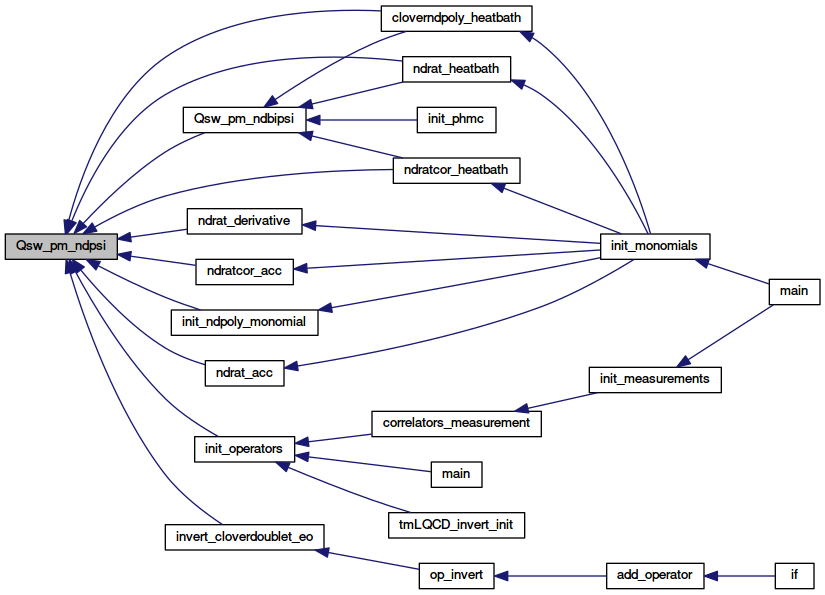
\includegraphics[height=7cm]{graphics/call_graph}
\end{frame}

\begin{frame}[fragile]{Funktionen: Definition}{Vorlesung \arabic{lecturecounter}}
\begin{block}{}
In der letzten Vorlesung hatten wir ein Programm entwickelt um eine Annäherung an die unendliche Summe
\begin{equation*}
  S=\sum_{n=0}^\infty x^n, \quad |x| < 1
\end{equation*}
zu bestimmen.
\end{block}
\begin{lstlisting}
const double x = 0.8;
double S = 0.0;
double xn = 1.0;
for( unsigned int n = 0; n < 1000; ++n ){  // max. 1000 Iterationen
  S = S + xn;
  if( xn < 1.0e-12 ){
    break;                        // aus der Schleife ausbrechen
  }                               // selbst wenn n < 1000
  xn = xn * x;
}
\end{lstlisting}
\textbf{Wir wollen nun mit einer Funktion die Berechnung auslagern und verallgemeinern.} (\verb|sum_xn_funktion.c|)
\end{frame}

\begin{frame}[fragile]{Funktionen: Funktionskopf und Signatur}{Vorlesung \arabic{lecturecounter}}
\begin{block}{}
  Eine Funktion wird dem Compiler bekannt gemacht, indem ihr Name und die Datentypen ihrer Argumente festgelegt werden. $\Rightarrow$ \emph{Funktionsdeklaration}
\end{block}

\begin{lstlisting}
RUECKGABETYP FUNKTIONSNAME( ARGUMENT1_TYP ARG1, ARGUMENT2_TYP ARG2,
                            ARGUMENT3_TYP ARG3 );
\end{lstlisting}
\begin{block}{Signatur}
  Dies nenn man auch die \emph{Signatur} der Funktion.
  {\footnotesize \verb| (FUNKTIONSNAME) ( ARGUMENT1_TYP, ARGUMENT2_TYP, ARGUMENT3_TYP ) | }
\end{block}
\textbf{Korrektur aus der Vorlesung:} Es darf nur eine Funktion mit dem Namen \texttt{FUNKTIONSNAME}.
\end{frame}

\begin{frame}[fragile]{Funktionen: Funktionsaufruf und Rückgabewert}{Vorlesung \arabic{lecturecounter}}
\begin{block}{}
Hat eine Funktion einen Rückgabewert, so kann man diesen beim Aufruf einer Variable zuweisen:
\begin{lstlisting}
double result = teilen( 8.0, 3.2 );  
\end{lstlisting}
\end{block}
\begin{block}{}
Man kann den Rückgabewert aber auch einer anderen Funktion als Argument übergeben:
\begin{lstlisting}
addieren( teilen(8.0, 3.2), 4.5 );
\end{lstlisting}
\begin{itemize}
  \item{Was macht dieser Code?} 
\end{itemize}
\end{block}
\begin{block}{}
Oder aber man ignoriert den Rückgabewert, wie wir es bei \texttt{printf([...])} getan haben (Gesamtzahl der geschriebenen Zeichen).
\end{block}
\end{frame}

\begin{frame}[fragile]{Funktionen: Deklaration und Definition}{Vorlesung \arabic{lecturecounter}}
\begin{block}{}
  Die \emph{Funktionsdeklaration} informiert den Compiler über die Existenz und Signatur einer Funktion
\begin{lstlisting}
double power( const double, const int );
\end{lstlisting}
\end{block}
\begin{block}{}
  Die \emph{Funktionsdefinition} beschreibt erst, wie diese Funktion ihre Aufgabe erfüllt.
\end{block}
Funktionsdeklarationen führen einerseits zu lesbarerem Code, finden aber andererseits Verwendung in der \emph{modularen Programmierung}, die wir in den nächsten Tagen kennenlernen werden.

\textbf{Erstmal ein Beispiel.} (\verb|funktion_deklaration.c|)
\end{frame}

\begin{frame}[fragile]{Funktionen: Rekursion}{Vorlesung \arabic{lecturecounter}}
  \begin{block}{Rekursion}
    Eine Funktion, die sich selbst aufruft, nennt man \emph{rekursiv}. Rekursion kann man oft nutzen, um Aufgaben auf fast magische Art und Weise zu lösen. Leider birgt Rekursion auch viele Gefahren.
  \end{block}
\begin{lstlisting}
TYP rekursion( TYP arg ){
  if( [...] ){ // Ziel erreicht!
    return arg;
  } else {
    return rekursion( arg ); // noch einmal tiefer verschachteln!
  }
}
\end{lstlisting}
   \textbf{Versuchen wir mal, unsere Summe rekursiv auszurechnen!} (\verb|sum_xn_rekursiv.c|)
\end{frame}
 
\begin{frame}[fragile]{\texttt{gdb} und \texttt{valgrind}}
\begin{block}{}
  Nanu, was ist denn da schiefgegangen? Ein Debugger, ist ein Programm, mit dem man Fehler in anderen Programmen versuchen kann nachzuvollziehen.
\end{block}
\begin{block}{Debugging-Symbole mit einbinden und Programm in \texttt{gdb} ausführen}
\begin{verbatim}
$ gcc -Wall -Wpedantic -g -ggdb -std=c99 \
  -o sum_xn_rekursiv_DEBUG sum_xn_rekursiv.c
$ gdb ./sum_xn_rekursiv_DEBUG
GNU gdb (Ubuntu 7.11.1-0ubuntu1~16.04) 7.11.1
(gdb) run
\end{verbatim}
\end{block}

\begin{block}{\texttt{valgrind}}
Ein weiteres nützliches Programm ist \texttt{valgrind}. Es ist eigentlich kein Debugger im eigentlichen Sinne, ist aber spezialisiert darauf, Speicherfehler zu erkennen.
\begin{verbatim}
$ valgrind ./sum_xn_rekursiv_DEBUG
\end{verbatim}
\end{block}
\end{frame}

\begin{frame}[fragile]{Statische Arrays}{Vorlesung \arabic{lecturecounter}}
  \begin{block}{}
    Oft brauchen wir viele Daten des gleichen Datentyps. Diese kann man praktisch in \emph{Arrays} abspeichern.
  \end{block}

\begin{lstlisting}
DATENTYP NAME[ANZAHL];
\end{lstlisting}
Hierbei muss, selbst in C99, \texttt{ANZAHL} fast immer eine numerische Konstante sein!

\begin{lstlisting}
double a[3];  // Array mit 3 double deklarieren

double b[3] = {1.0, 2.3, 9.9};  /* Array mit 3 double deklarieren
                                   und initialisieren */

double c[4] = {4.5, 7.3}; /* Die ersten beiden Elemente mit 
                             4.5 und 7.3 initialisieren,
                             alle anderen werden mit 0.0 
                             initialisiert */
                                   
a[1] = 0.0001; // 0.0001 im zweiten Element von v abspeichern
\end{lstlisting}
\textbf{$\Rightarrow$ Wir möchten nun für unsere Annäherung an die unendliche Summe alle Terme abspeichern und ausgeben!} (\verb|sum_xn_alleterme.c|)
\end{frame}

\begin{frame}[fragile]{Mini-Intro: Texteingabe}{Vorlesung \arabic{lecturecounter}}
\begin{block}{Der Adressoperator \texttt{\&}}
  Für jede Variable, jedes Datentyps, gibt \texttt{\&} die Speicheradresse der Variable zurück. (Um genauer zu sein, ist der Rückgabewert ein Zeiger auf ein Objekt des ensprechenden Datentyps)
\end{block}
\begin{block}{Eingabe mit \texttt{scanf}}
  Die Funktion \texttt{scanf} kann als umgekehrtes \texttt{printf} verstanden werden.
\end{block}
\begin{lstlisting}
int ganzzahl; double dezimalzahl;
scanf("%d %lf",&ganzzahl, &dezimalzahl);
\end{lstlisting}
\textbf{Probieren wir mal, ob wir so unser Summenprogramm weiter verallgemeinern können.} (\verb|test_scanf.c| und \verb|sum_xn_eingabe.c|)
\end{frame}

\begin{frame}[fragile]{Preview: Zeiger auf Daten}{Vorlesung \arabic{lecturecounter}}
\begin{block}{Zeigervariablen}
  Eine Zeigervariable speichert die Adresse einer Variable für einen bestimmten Datenyp.
\end{block}
\begin{block}{Dereferenzierungsoperator \texttt{*}}
  Dieser Operator gibt Zugriff zu den Daten, auf die der Zeiger zeigt.
\end{block}
$\Rightarrow$ \textbf{Tafelbild +} (\texttt{zeiger\_preview.c})
\end{frame}

\stepcounter{lecturecounter}

\begin{frame}[fragile]{Fragen zu Vorlesung 2}{Vorlesung \arabic{lecturecounter}}
  \begin{itemize}
    \item{Platzhalter in \texttt{printf}}
    \item{C-Programme als Funktionssammlungen}
    \item{Funktionen: Kopf, Signatur, Aufruf, Deklaration, Definition, Rückgabewert, Rekursion}
    \item{Debugger Mini-Mini-Intro}
    \item{Statische Arrays}
    \item{Texteingabe mit \texttt{scanf}}
    \item{Preview: Zeiger}
  \end{itemize}
\end{frame}

\begin{frame}[fragile]{Zeiger}{Vorlesung \arabic{lecturecounter}}
  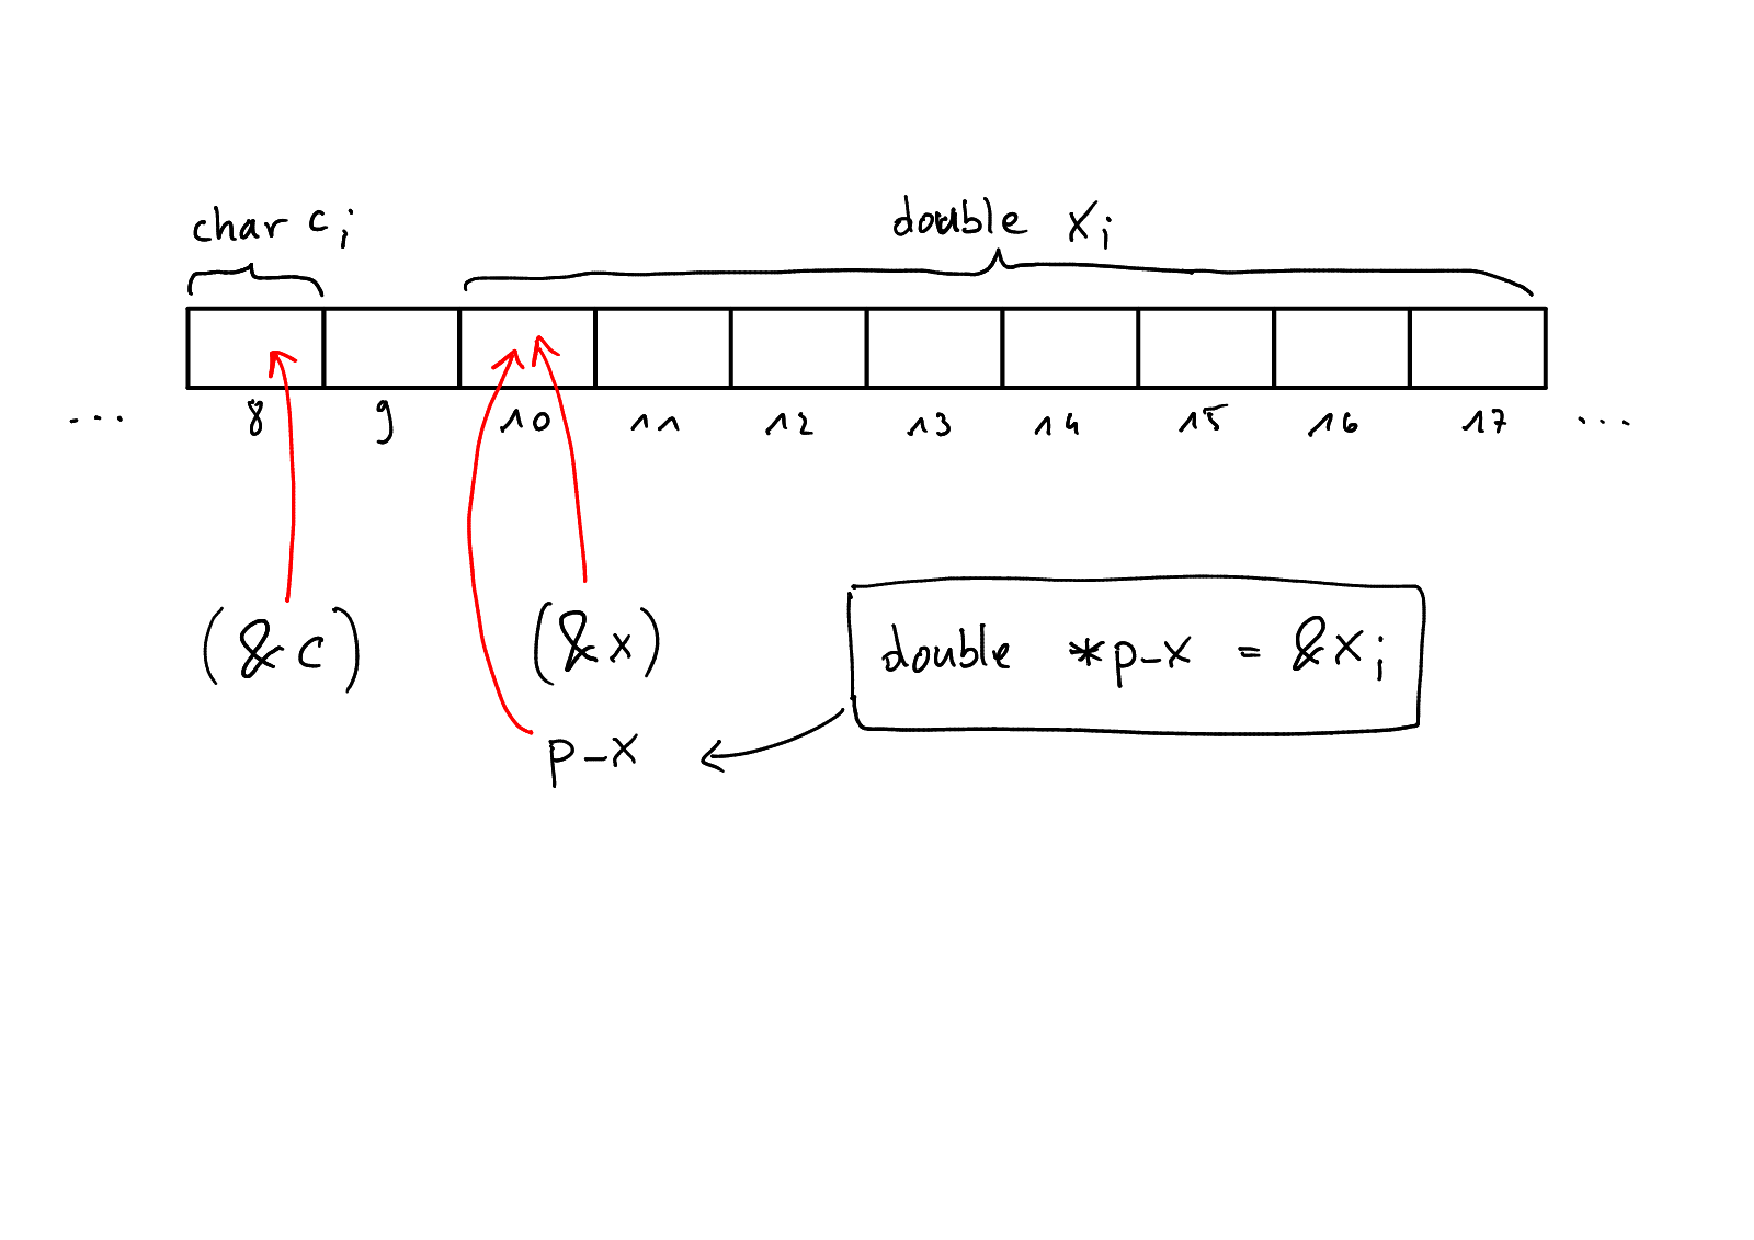
\includegraphics[width=\textwidth,page=1,trim=0 7cm 0 2cm,clip=true]{graphics/c_kurs_tafel}
  \begin{block}{}
    Zeiger sind Datentypen, welche die Adresse einer Variable oder, allgemein, eines Speicherbereichs darstellen.
  \end{block}
  $\Rightarrow$ (\texttt{zeiger\_demo.c}) und Tafelbild
  \begin{block}{}
    Ein \texttt{NULL}-pointer zeigt auf gar nichts.
  \end{block}
\end{frame}

\begin{frame}[fragile]{Arrays, Zeiger und einfache Zeigerarithmetik}{Vorlesung \arabic{lecturecounter}}
  \begin{block}{}
    Statische Arrays sind spezielle Speicherbereiche, für die der Compiler einen Standardzeiger setzt. Dieser Zeiger ist der Name des Arrays.
  \end{block}
\begin{lstlisting}
int a[4];   /* 'a' hat Datentyp (int*) und zeigt  
               auf ein Array des Typs (int) */
int *b = a; /* 'b' hat auch den Datentyp (int*) und zeigt jetzt
               auf den gleichen Speicherbereich wie 'a' */
\end{lstlisting}
\begin{block}{}
  Strikt gesehen sind arrays und Zointer (\emph{pointer}) auf Daten des gleichen Datentyps aber nicht identisch!
\end{block}
 $\Rightarrow$ (\texttt{zeiger\_array\_demo.c}) und Tafelbild

\end{frame}

\begin{frame}[fragile]{Zeichenketten}{Vorlesung \arabic{lecturecounter}}
  \begin{block}{}
    \begin{itemize}
      \item{Die Manipulation von Zeichenketten (auch \emph{strings}) ist in vielen Programmen von zentraler Bedeutung, z.B. um Dateinamen für Ausgabedateien zu setzen.}
      \item{In C werden einfache strings in \texttt{char}-Arrays gespeichert. Da \texttt{char} nur 1B groß ist, stehen einem bloß 255 verschiedene Zeichen zur Verfügung.}
      \item{Strings werden in C \emph{null-terminiert}: Am Ende eines Strings steht ein spezielles Zeichen, welches man auch selbst mit '\textbackslash 0' einfügen kann.}
      \item{Ein C String ist also ein \texttt{char}-Array der Länge $n$ für maximal $n-1$ Zeichen.}
    \end{itemize}
  \end{block}
  \begin{lstlisting}
    // dies ist ein string
    char begruessung[20] = "Hallo, Welt!\n";
    printf("%s", begruessung);
  \end{lstlisting}
  $\Rightarrow$ (\verb|test_strings.c|)
\end{frame}

\begin{frame}[fragile]{Zeichenketten bearbeiten: \texttt{snprintf}}{Vorlesung \arabic{lecturecounter}}
  \begin{block}{}
    \begin{itemize}
      \item{C enthlält viele Funktionen zur Manipulation von Zeichenketten. Fast alle sind unsicher.}
      \item{Es gibt eine Ausnahme: \texttt{snprintf}}
    \end{itemize}
  \end{block}
  (\verb|unsichere_Zeichenketten.c|)  und (\verb|test_snprintf.c|)
\end{frame}

\begin{frame}[fragile]{\emph{Pass-by-reference}: Zeiger an Funktionen übergeben}{Vorlesung \arabic{lecturecounter}}
  \begin{block}{}
    Wie wir gesehen haben, existieren Variablen in C -- sofern es sich nicht um globale Variablen handelt -- nur innerhalb eines Blocks. Aus Effizienzgründen ist es oft aber unratsam, Kopien großer Datenstrukturen hin- und herzuschieben.
  \end{block}
  Wir können aus der Funktion \texttt{inkrement}, nicht einfach so auf \texttt{x} aus der Funktion \texttt{main} zugreifen.
  \begin{lstlisting}
int inkrement(int n){
  x += n; // Fehler: 'inkrement' kennt 'x' nicht!
}  
int main(void){
  int x = 22;
  inkrement(4); // Fehler: 'inkrement' kennt 'x' nicht!
  return 0;
} 
\end{lstlisting}
\vspace{-0.4cm}
  \begin{block}{}
    Mithilfe von Zeigern, können wir Funktionen direkt auf Daten anwenden, welche in einem anderen Block deklariert wurden. (wie bei \texttt{scanf} gemacht)
  \end{block}
  $\Rightarrow$  nächste Folie
\end{frame}

\begin{frame}[fragile]{\emph{Pass-by-reference}: Zeiger an Funktionen übergeben}{Vorlesung \arabic{lecturecounter}}
  \begin{block}{}
    Übergeben wir die Adresse von \texttt{x} an die Funktion, hat diese direkten Zugriff auf die Variable \texttt{x} aus der \texttt{main}-Funktion.
  \end{block}
  \begin{lstlisting}
int inkrement(int *z_x, int n){
  *z_x += n;
}  
int main(void){
  int x = 22;
  inkrement(&x, 4); // x wird von 'inkrement' um 4 inkrementiert
}
\end{lstlisting}
\vspace{-0.4cm}
  \begin{block}{}
    Das können wir auch anhand unserer Summenfunktion zeigen:
  \end{block}
  $\Rightarrow$ (\verb|sum_xn_by_reference.c|)
\end{frame}

\begin{frame}[fragile]{Kommandozeilenargumente}{Vorlesung \arabic{lecturecounter}}
\begin{block}{}
  In unseren Programmen haben wir bisher
\end{block}
\begin{lstlisting}
  int main(void){ [...] } 
\end{lstlisting}
\begin{block}{}
  geschrieben. \texttt{void} bedeutet leer oder auch ungültig. Wir haben damit darauf hingedeutet, dass unsere \texttt{main}-Funktion keine Argumente entgegennimmt.
  \begin{itemize}
    \item{Der \texttt{main}-Funktion werden aber vom Betriebssystem Argumente übergeben: die Kommandozeilenargumente}
  \end{itemize}
\begin{verbatim}
$ ./programm arg0 arg1 arg2
\end{verbatim}
\begin{lstlisting}
int main(int argc, char **argv){
  [...]
}
\end{lstlisting}

\end{block}
$\Rightarrow$ (\texttt{test\_argc.c})
\end{frame}

\begin{frame}[fragile]{Kommandozeilenargumente auslesen}{Vorlesung \arabic{lecturecounter}}
  \begin{block}{}
    \begin{itemize}
      \item{Bei \texttt{**argv} (oder auch \texttt{*argv[]}) handelt es sich um ein Array von Strings (ein Array von \texttt{char}-Arrays).}
      \item{C bietet einige Funktionen, die es erlauben aus Strings andere Datentypen auszulesen.}
      \item{\texttt{sscanf} ist eine mit \texttt{scanf} verwandte Funktion}
      \item{Für Kommandozeilenargumente ist es oft praktischer einfachere Funktionen zu nutzen.}
      \begin{itemize}
        \item{\verb|atoi, atof, strtod, strtol, strtoul, strtoull|}
      \end{itemize}
    \end{itemize}
  \end{block}
  $\Rightarrow$ (\texttt{test\_read\_argv.c})
\end{frame}

% \stepcounter{lecturecounter}
% \begin{frame}[fragile]{Fragen zu Vorlesung 3}{Vorlesung \arabic{lecturecounter}}
% \end{frame}
% 
% \begin{frame}[fragile]{Modulare Programmierung}{Vorlesung \arabic{lecturecounter}}
% \begin{block}{}
%   \begin{itemize}
%     \item{Einzelne Funktionen können in C in separaten Quelltextdateien stehen und unabhängig voneinander kompiliert werden.}
%     \item{Wir können dies wieder anhand unserer Summenfunktion darstellen.}
%   \end{itemize}
% \begin{enumerate}
%   \item{Funktionen in separate Dateien auslagern}
%   \item{Einzelne Module kompilieren}
%   \item{Module zu Programm verlinken}
% \end{enumerate}
% \end{block}
% \begin{itemize}
%   \item{ \textt{sum\_xn(...)} $\rightarrow$ \texttt{sum\_xn.c} }
%   \item{
% \end{itemize}
% 
% \end{frame}
% 
% \begin{frame}[fragile]{Compiler und Linker}{Vorlesung \arabic{lecturecounter}}
% \end{frame}
% 
% \begin{frame}[fragile]{Der C-Präprozessor}{Vorlesung \arabic{lecturecounter}}
% \begin{block}{}
%   \begin{itemize}
%     \item{Wir haben bisher einen Teil des Kompilierprozesses ausgelassen: den Präprozessor.}
%     \item{Bevor der Compiler seinen Dienst verrichtet, wird der Quelltext vom Präprozessor bearbeitet.}
%   \end{itemize}
% \end{block}
% \begin{block}{Präprozessorkonstanten und Makros}
%   Makros sind Platzhalter für Codeblöcke, welche vom Präprozessor beim Durchlauf in den Quelltext eingefügt werden.
% \end{block}
% \end{frame}
% 
% \begin{frame}[fragile]{Header-Dateien}{Vorlesung \arabic{lecturecounter}}
% Wir haben Header-Dateien
% \begin{lstlisting}
%   
% \end{lstlisting}
% \end{frame}
% 
% \begin{frame}[fragile]{Ein echtes modulares Programm}{Vorlesung \arabic{lecturecounter}}
% 
% \end{frame}
% 
\end{document}